\subsection{Use Case}

\subsubsection{Use Case Diagram}
	
	
\begin{figure}[h]

	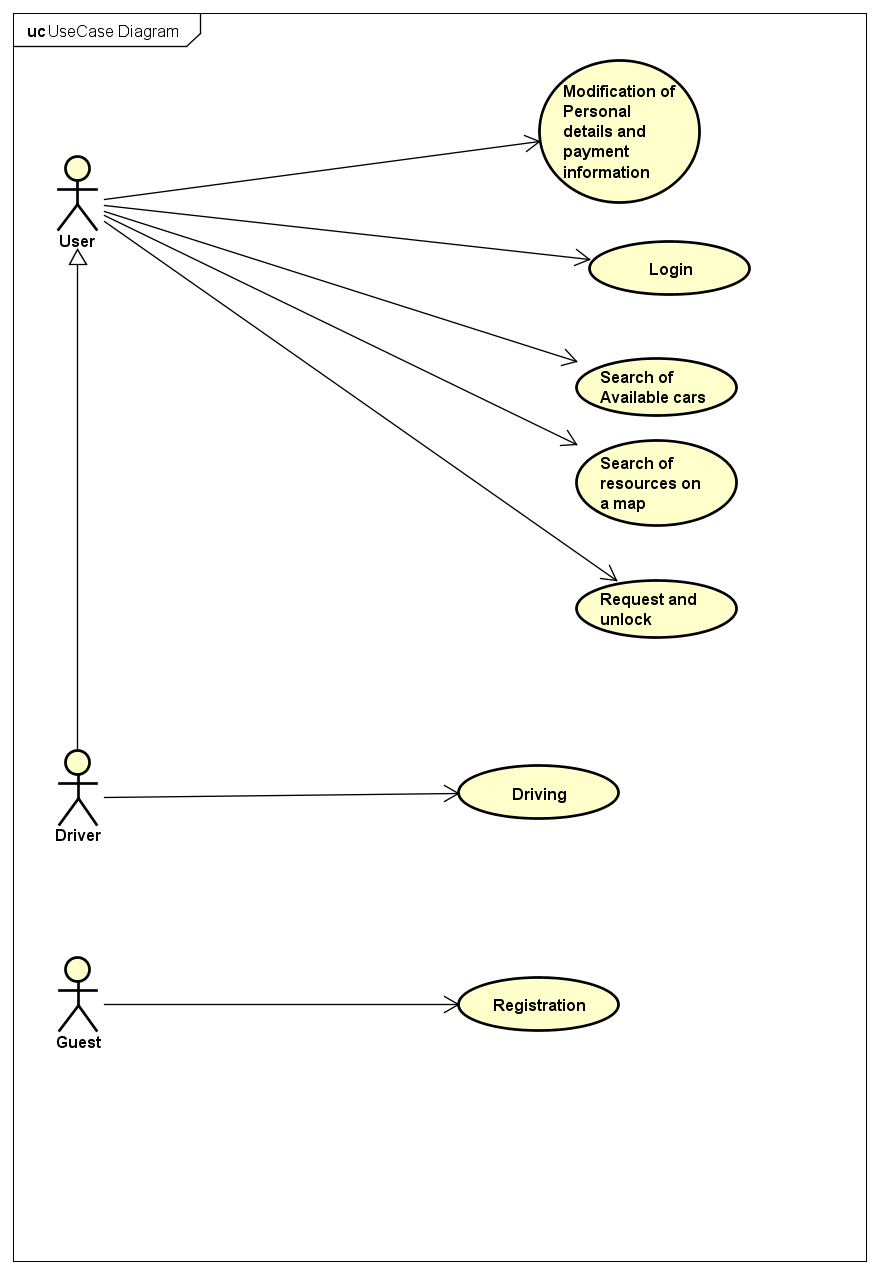
\includegraphics[width=300px, height=400px]{img/UseCase_Diagram}
	
\end{figure}
	
\pagebreak



\subsubsection{User Registration}

	% example \usecase{name}{actor}{goal}{precondition}{post condition}{flow}{exception}


	
	
	
	\usecase{User Registration}
				{Guest}
				{\goal{1}}
				{Guest hasn't registered to the webapp yet.}
				{Guest is signed-up and promoted to ``PowerEnJoy'' User.}
				{
					\begin{enumerate}
						\item Guest accesses to the webapp or the mobile application
						\item Guest clicks on ``Sign Up'' button
						\item Guest fill Sign-up form fields, entering\\
						-Name\\
						-Surname\\
						-Email address\\
						-Password\\
						-Telephone Number\\
						-Driving License number
						\item Guest accepts the term of use
						\item Guest clicks on ``Confirm'' button\end{enumerate}
				}
				{-}
				{
				\begin{enumerate}
					\item At least one field is empty when the guest has confirmed. The system shows again the 									registration form, showing in addition a message advising the guest that she missed a field. 
					\item At least one field is invalid when the guest has confirmed. The system shows again the 									registration form, indicating the invalid field.
					\item Entered email is already associated to another account. The system shows again the 									registration form, showing in addition a message advising the guest that the email is already 								associated to another account.
					
					
					
					\end{enumerate}
				}
\pagebreak


\subsubsection{User Login}\label{login}

\usecase{User Login}
{User}
{\goal{2}}
{User has signed-up as PowerEnJoy User.}
{User is redirected to personal area.}
{
	\begin{enumerate}
		\item User accesses to the webapp or the mobile application
		\item User clicks on ``Log-in' button
		\item User fills username and password fields of Log-in form
		\item User clicks on ``Submit'' button
	\end{enumerate}
}
{-}
{
	\begin{enumerate}
		\item Invalid username and/or password. User is redirected by the system again to the page of Login form.
		\item At least one field is empty. User is redirected by the system again to the page of Login form.
	\end{enumerate}
}

\begin{figure}[h]

	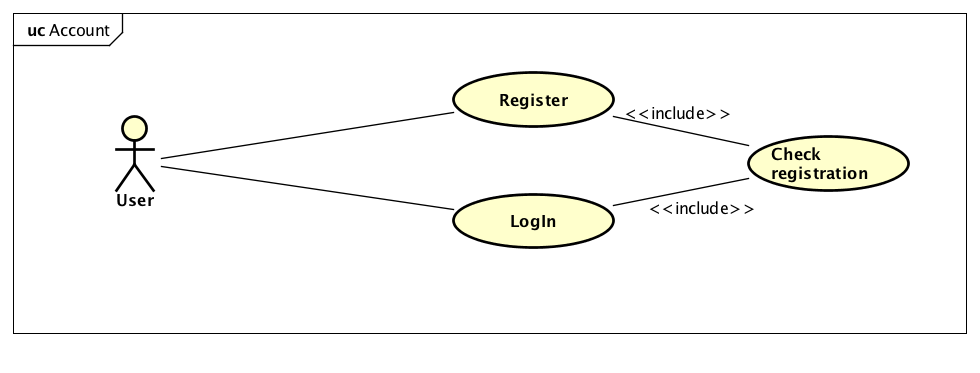
\includegraphics[width=380px]{img/usecase_login_registration}
	\caption{Use Case Login and Registration procedure. Refer to Goal 1 and 2}
\end{figure}
\pagebreak


\subsubsection{Modification of personal details and payment information}
\usecase{Modification of personal details and payment information}
{User}
{\goal{3}}
{User is logged in}
{User is redirected to the modifications area where he can modify his personal information}
{
\begin{enumerate}
	\item User clicks on ``Personal Details' button in his personal area. A page with the personal data of the user is shown'
	\item User clicks on ``Modify Data'' button. A form for modifications is shown
	\item User fills fields he wants to modify
	\item User clicks on ``Confirm'' button
	\item User is redirected to his personal area
\end{enumerate}
}
{-}
{-}
\pagebreak


\subsubsection{Search of available cars}\label{search}
\usecase{Search of available cars}
{User}
{\goal{4}}
{User is logged in}
{User is redirected to a page with the list of the available cars}
{
\begin{enumerate}
	\item User clicks on ``Search a car'' button in his personal area. A form is shown
	\item User select a distance from the ``Distance from your position'' field
	\item User clicks on ``Confirm'' button
	\item User is redirected to a page showing the available cars
\end{enumerate}
}
{
\begin{itemize}
\item Different flow from step 2:
	\begin{enumerate}
	\item[2] User write an address in the ``Address'' field 
	\item[3] User clicks on ``Confirm'' button
	\item[4] User is redirected to a page showing the available cars
 
\end{enumerate}

\end{itemize}


}
{
\begin{enumerate}
\item There aren't available cars within the distance set 
\item There aren't available cars near the address set
\end{enumerate}
}
\pagebreak

\subsubsection{Search of resources on a map}\label{search2}
\usecase{Search of resources on a map}
{User}
{\goal{5}}
{User is logged in}
{User is redirected to a page with a map where resources (available cars, safe areas, special parking areas)  are shown}
{
\begin{enumerate}
	\item User clicks on ``Search resources on the map'' button. A form is shown
	\item User select a distance from the ``Distance from your position'' field
	\item User clicks on ``Confirm'' button
	\item User is redirected to a page showing the resources on a map.
\end{enumerate}
}
{
\begin{itemize}
\item Different flow from step 2:
	\begin{enumerate}
	\item[2] User write an address in the ``Address'' field 
	\item[3] User clicks on ``Confirm'' button	
	\item[4] User is redirected to a page showing the resources on a map.
 
\end{enumerate}

\end{itemize}


}
{
\begin{enumerate}
\item There aren't available cars within the distance set 
\item There aren't available cars near the address set
\end{enumerate}

}
\pagebreak


\subsubsection{Request and Unlock}\label{request}
\usecase{Request and Unlock}
{User}
{\goal{6} \newline \goal{10} \newline \goal{11}}
{User is logged in and has searched a car (\ref{search}, \ref{search2}}
{The car requested is reserved for the user}
{
\begin{enumerate}
	\item User selects a car from the list. 
	\item A page with information about the car (battery level, model, engine size, autonomy in kilometers) is shown
	\item User clicks the ``Request'' Button''
	\item The car is reserved for the user
	\item User reaches the car and is less than 3 meters far from the car
	\item User unlocks the car clicking on the ``Unlock'' button in the application

\end{enumerate}
}
{
\begin{itemize}
\item Steps 1 is different:
	\begin{enumerate}
	\item[1] User select a car on the map.   
	\end{enumerate}
\item Different flow from step 5:
	\begin{enumerate}
	\item[5] An hour passes without the User unlocking the car
	\item[6]The system charges the User with an extra fee of 1 euro
	\item [7]The system cancels the request and makes the requested car available again
	\end{enumerate}
\end{itemize}


}
{
\begin{enumerate}
\item The car selected has been requested by another user before the User has clicked on the ``Request'' button.
\end{enumerate}
}
\pagebreak


\subsubsection{Driving}
\usecase{Driving}
{Driver}
{\goal{7} \newline \goal{9} \newline \goal{12} \newline \goal{13}}
{Driver is logged in and has searched, requested and unlocked a car}
{-}
{
\begin{enumerate}
\item Driver enters the car, eventually also other passengers enter the car
\item Driver starts driving
\item The system detects the number of passengers
\item The screen shows a map with the position of the car, the safe areas and special parking areas near the car position
\item The screen shows the money to be charged up to the current moment
\item The system charges the standard fee every minute.
\item Driver parks and exit the car and, if any, the other passengers exit the car
\item The system locks the car
\item The system detects the level of the battery
\item The system detects if the car has been plugged in a power grid
\item The system detects the position of the left car
\item The system applies a discount on the ride of the:
	\begin{itemize}
	\item 10\%, if it has detected the presence of at least two other passengers in addition to the driver during the travel
	\item 20\%, if it has detected that the car was left with no more than the 50\% of the battery empty
	
	\end{itemize}
\item The system charges the 30\% more on the last ride if it detects that the car has been left more than 3 km far
	from the nearest power grid station
	\end{enumerate}
\item The system takes the money from the User, using his selected payment method
}
{
	\begin{itemize}
	\item Before the last step, the system detects the presence of at least two other passengers in addition to the driver during the 		         travel and so applies a 10\% discount on the ride
	\item Before the last step, the system detects that the car was left with no more than the 50\% of the battery empty and so 			         applies a 10\% discount on the ride
	\item At step 7 the Driver parks the car in a special parking area and plugs the car into the power grid. Before the last step the 
	         the system detects that the car has been plugged into the power grid and so applies a 20\% discount on the ride
	\item While driving the Driver exits the city area. So:
		\begin{enumerate}
		\item An acoustic signal is emitted by the screen
		\item A message is shown on the screen, warning the Driver that he has exited the city area
		\item The system charges the 100\% more than the standard fee every minute until the driver re-enters in the city area
		\end{enumerate} 
	\end{itemize}

}
{-}
\todo{C'è da fare chiarezza su city area/ safe area}

\section{Sequence Diagrams}




\section{Scenarios}

\subsection{Scenario 1}

Andrew is a student. Because in his home city there aren't the courses he wants to attend, he moves to another city. There he rents a flat with other students. During the week he doesn't need any mean of transport and travels only on foot,  because his house is very near to the university. In the weekend Andrew wants to have some fun with his friends, but	unfortunately the areas with the coolest bars are far from his house and at night there aren't public transports going to those area. Futhermore neither he or his friends have a car, because they are all out of their home towns. So Andrew uses his Power EnJoy application, searches a car near his address, reserves a car, reaches it and drives till his favourite fun area, carrying with him some of his friends.

\subsection{Scenario 2}

It's Friday night and Bob have to go out with his girlfriend. Unfortunately his parents are away and have the car with them, so Bob searches a car near his home using Power EnJoy application. He sees on the map that there is only one car near his house and that its autonomy allows him only to reach his girlfriend's house. He looks for a special parking area near his girlfriend's house and finds one.
So he decides to go to that special parking area, leave there the car, plug it into the power grid and request again for that car. Then he waits there for his girlfriends, having enough charge when she arrives to go downtown.

\subsection{Scenario 3}

Jim and Kate are two young tourists. They walked a lot all the day and so now they want to find an easy way to go to their hotel.
Jim his registered to the Power EnJoy car-sharing service, so his reserves and picks up a car. They decide to park the car near the hotel, but when they're going to do that, they see a message telling that they are more than 3 km far from the nearest power station. Because Jim knows would have to pay more because of that and he hasn't a lot of money left, he decides to park nearer to a power station.
    




\FloatBarrier


